

The second geometric model tested is the \emph{Gaussian model}. The aim of this model was to reproduce a polarization morphology that transitions from being aligned with the minor axis of the disk at the centre to becoming more azimuthal towards the outer parts of the disk. This is based on the expectation that the emission from the inner region is optically thick \citep{Kataoka_2015}, with optical thickness decreasing towards the outer edge of the disk. 


To achieve this, we used a rotated 2-dimensional flat-topped Gaussian model with three free parameters: $\phi$, $a$ and $b$. The Gaussian was calculated using the equation :
\begin{equation}
W_{\text{Uniform}} =  I_0 
\exp\left[-\half \left(\left|\frac{X_{M}}{\sigma_M}\right|^\phi + \left|\frac{Y_{m}}{ \sigma_m}\right|^\phi\right)\right],
    \label{eq: gaussian_eq}
\end{equation}
\noindent where $I_0$, the peak value, was calculated using the equation:
\begin{equation}
    I_0 = \frac{1} {\sigma_m \sigma_M \sqrt{2\pi}}.
    \label{eq: Gaussian_model_I0}
\end{equation}

\noindent In Equation \ref{eq: gaussian_eq}, $\phi=2$ corresponds to a standard 2D Gaussian, while $\phi>2$ produces a flat-topped Gaussian. Table \ref{tab: gaussian_model_info} lists the parameters and the ranges we tested. The tested values of $a$ and $b$ control the widths of the Gaussian model (major and minor axes of the Gaussian, respectively), with each treated as the FWHM and converted to standard deviations using Equation \ref{eq: FWHM_to_sigma}. Additionally, a condition of $b$ $\leqq $ $a$ was required to ensure the minor axis was smaller than the major axis. 


% \begin{equation}
% f(x) = A \exp{\left(-\left(\frac{(x-x_0)^2}{2\signa_X^2}\right)^P\right)}
%     \label{eq: super-Gaussian}
% \end{equation}
% \question{do I need to cite this? I got it from Wikipedia.}


\begin{table}[h!]
\centering
\caption{Summary of parameters and tested values in the Gaussian model.  }
\begin{tabular}{lll}
\toprule
\textbf{Property} &
\textbf{Meaning} &
\textbf{Tested Values}  \\
\midrule

$\phi$
& super-Gaussian exponent
& 2, 3, 4, 5, 6, 7\\


$a$ (pixels)
& major axis of Gaussian
& 10, 20, 30, 40, 50\\

$b$ (pixels)
& minor axis of Gaussian
& 10, 20, 30, 40, 50\\

\bottomrule
\end{tabular}
\label{tab: gaussian_model_info}
\end{table}


The Gaussian was rotated to align with the major axis of the disk, using the position angle of the disk (\PAns) given in Table \ref{tab: source_info}. The coordinates ($x, y$) were shifted with respect to the centre of the disk ($x_c, y_c$) and then rotated:
\begin{equation}
\begin{pmatrix}
X_M \\
Y_m
\end{pmatrix}
=
\begin{pmatrix}
\cos(\PAeq) & -\sin(\PAeq) \\
\sin(\PAeq) & \cos(\PAeq)
\end{pmatrix}
\begin{pmatrix}
x - x_c \\
y - y_c
\end{pmatrix}.
\label{eq:rotated_coordinates}
\end{equation}





\noindent The Gaussian was normalized to a maximum of 1 so that it could be used as a pixel weight. Equation \ref{eq: gaussian_eq} creates a map that specifies the weights for the Uniform polarization region of the disk, where the weight is 1 at the centre and drops to zero with radius.  We use 1 - \Wuni to give the weight for the azimuthal polarization morphology. These two maps act as our weights, rather than a constant like in the ratio model. 


The weighted \SQ and $U$ were calculated by:
\begin{equation}
\begin{aligned}
Q_{\text{Gaussian}}
    &= \WuniEQ \,Q_{\text{Uni}}
     + (1 - \WuniEQ)\,Q_{\text{Azi}}, \\
U_{\text{Gaussian}}
    &= \WuniEQ\,U_{\text{Uni}}
     + (1 - \WuniEQ)\,U_{\text{Azi}},
\end{aligned}
% \label{eq:50U50A}
\end{equation}

\noindent As in the ratio model, the maps of $Q_{\text{Gaussian}}$ and $U_{\text{Gaussian}}$ were used to calculate the position angle (Equation \ref{eq: PA}). Figure \ref{fig: Methods/GaussianExamples} shows two example Gaussian weight maps with polarization vectors overlaid.  The values of $\phi$, $a$, and $b$ are given in the lower-left corner.  The vector sampling is selected to match the \bfour data.


\begin{figure}[htbp]
  \centering
  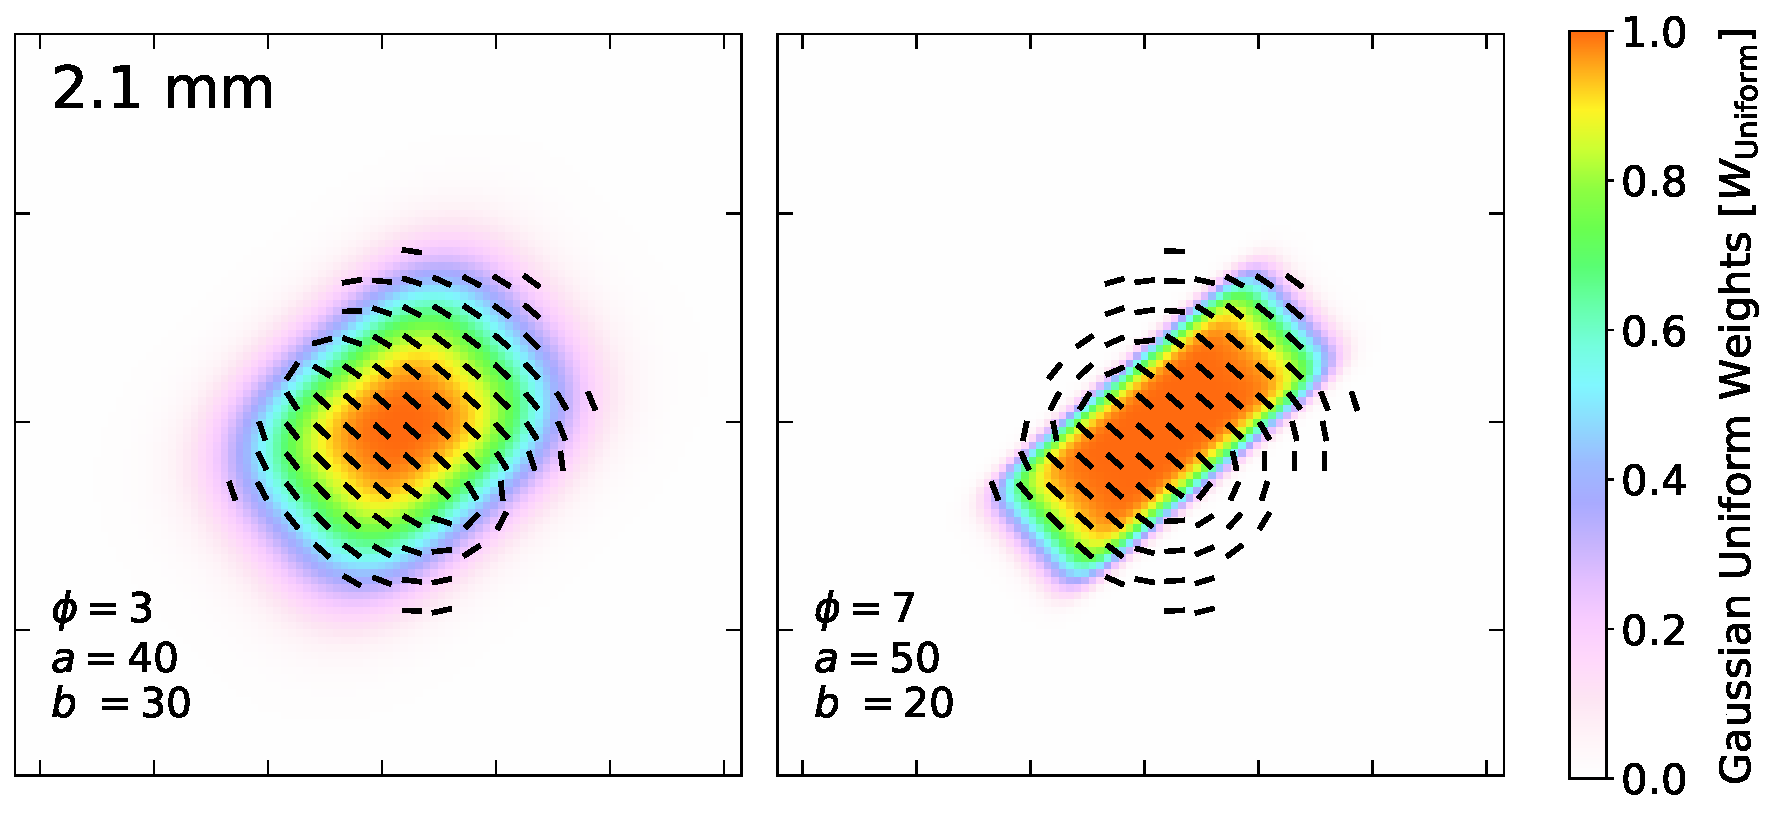
\includegraphics[width=0.8\textwidth]{WRITEUP_AND_IMAGES/IMAGES/WRITEUP/Gaussian/CustomExamples_B4.pdf}
  \caption{Two examples of the Gaussian weights for selected values of $\phi$, $a$ and $b$.}
  \label{fig: Methods/GaussianExamples}
\end{figure}





% ----------------------------------------------------------




For the Gaussian model, Table \ref{tab:gaussian_top5} presents the five best-fitting cases (out of 150 tested) with the best-fit model highlighted in bold.  Figure \ref{fig: GaussianBestGrid} compares the observed and model vectors for the best-fit models at each wavelength. 




\begin{figure}[htbp]
  \centering
  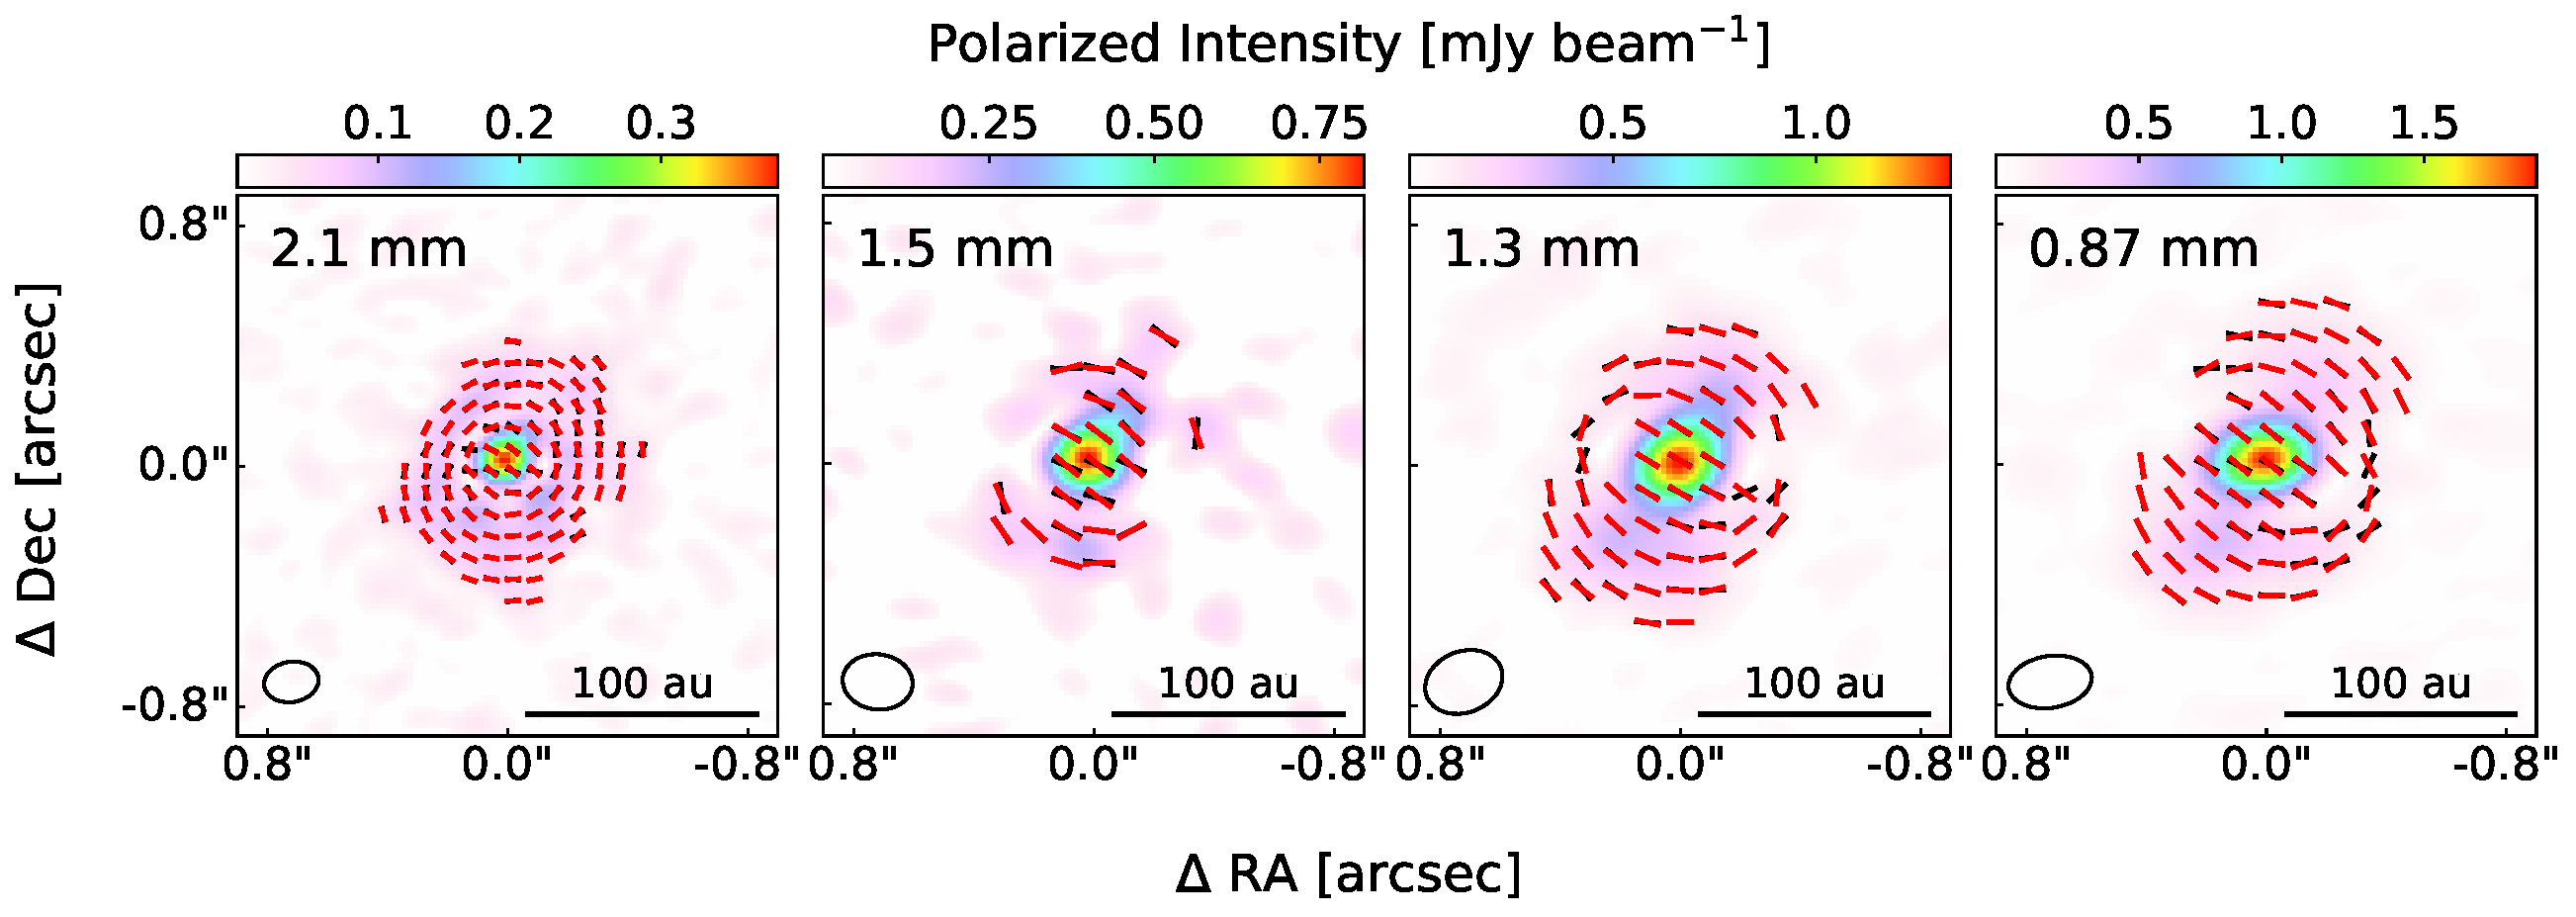
\includegraphics[width=0.99\textwidth]{WRITEUP_AND_IMAGES/IMAGES/WRITEUP/Gaussian/Best_grid_Delta.pdf}
  \caption{Same as Figure \ref{fig: RatioBestGrid}, but for the best-fit Gaussian models. The corresponding best-fit Gaussian models are listed Table \ref{tab:gaussian_top5}.}
  \label{fig: GaussianBestGrid}
\end{figure}





% This was updated to Band 5 robust = -1 on July 18th
% Needs updating if we change how we calculate chi-squared
% Band 4 and Band 7 nterms 2

\begin{table}[h!]
\centering
\caption{Top give Gaussian model fits at each wavelength, sorted by $\chi^2_{reduced}$. The best fit at each wavelength is shown in bold.}
\begin{tabular}{c ccc c}
\toprule
\textbf{Wavelength} & $\boldsymbol{\phi}$ & $\boldsymbol{a}$ & $\boldsymbol{b}$ &  $\boldsymbol{\chi^2}$ \\
\midrule

\textbf{\bfour} 
& \textbf{7} & \textbf{20} & \textbf{10} & \textbf{26.70} \\
 & 6 & 20 & 10 & 26.79 \\
 & 5 & 20 & 10 & 26.95 \\
 & 4 & 20 & 10 & 27.30 \\
 & 3 & 20 & 10 & 28.04 \\

\midrule

\textbf{\bfive} 
& \textbf{4} & \textbf{30} & \textbf{20} & \textbf{13.88} \\
 & 5 & 30 & 20 & 13.92 \\
 & 6 & 30 & 20 & 14.09 \\
 & 3 & 30 & 20 & 14.16 \\
 & 7 & 30 & 20 & 14.30 \\

\midrule

\textbf{\bsix} 
& \textbf{4} & \textbf{30} & \textbf{30} & \textbf{8.08} \\
 & 5 & 30 & 30 & 8.09 \\
 & 6 & 30 & 30 & 8.19 \\
 & 7 & 30 & 30 & 8.33 \\
 & 3 & 30 & 30 & 8.41 \\

\midrule

\textbf{\bseven} 
& \textbf{6} & \textbf{40} & \textbf{30} & \textbf{38.56} \\
 & 5 & 40 & 30 & 38.59 \\
 & 7 & 40 & 30 & 38.69 \\
 & 6 & 30 & 30 & 38.86 \\
 & 7 & 30 & 30 & 38.88 \\

\bottomrule
\end{tabular}
\label{tab:gaussian_top5}
\end{table}



  


From the results in Table \ref{tab:gaussian_top5}, the values of $a$ and $b$ are consistent among the top five models at each wavelength, but the values differ between wavelengths. This indicates that, within each wavelength, these values provide a good fit among the tested values. For simplicity, the area of the Gaussian is defined as:
\begin{equation}
A = a \cdot b.
    \label{eq: GaussianArea}
\end{equation}
\noindent A larger value of $A$ corresponds to a larger area of uniform morphology. For\bfourNS, \bfiveNS, \bsiNS, and \bsevenNS the corresponding areas are 200, 600, 900, 1200 pixels$^2$, respectively. The increase in area as wavelength decreases indicates the uniform morphology contributes over a larger region of the disk at shorter wavelengths. This can be seen in Figure \ref{fig: gaussian_best_map_w_uniform}, showing the Gaussian shape ($W_{\text{Uniform}}$) for the best-fit model at each wavelength.


\begin{figure}[htbp]
  \centering
  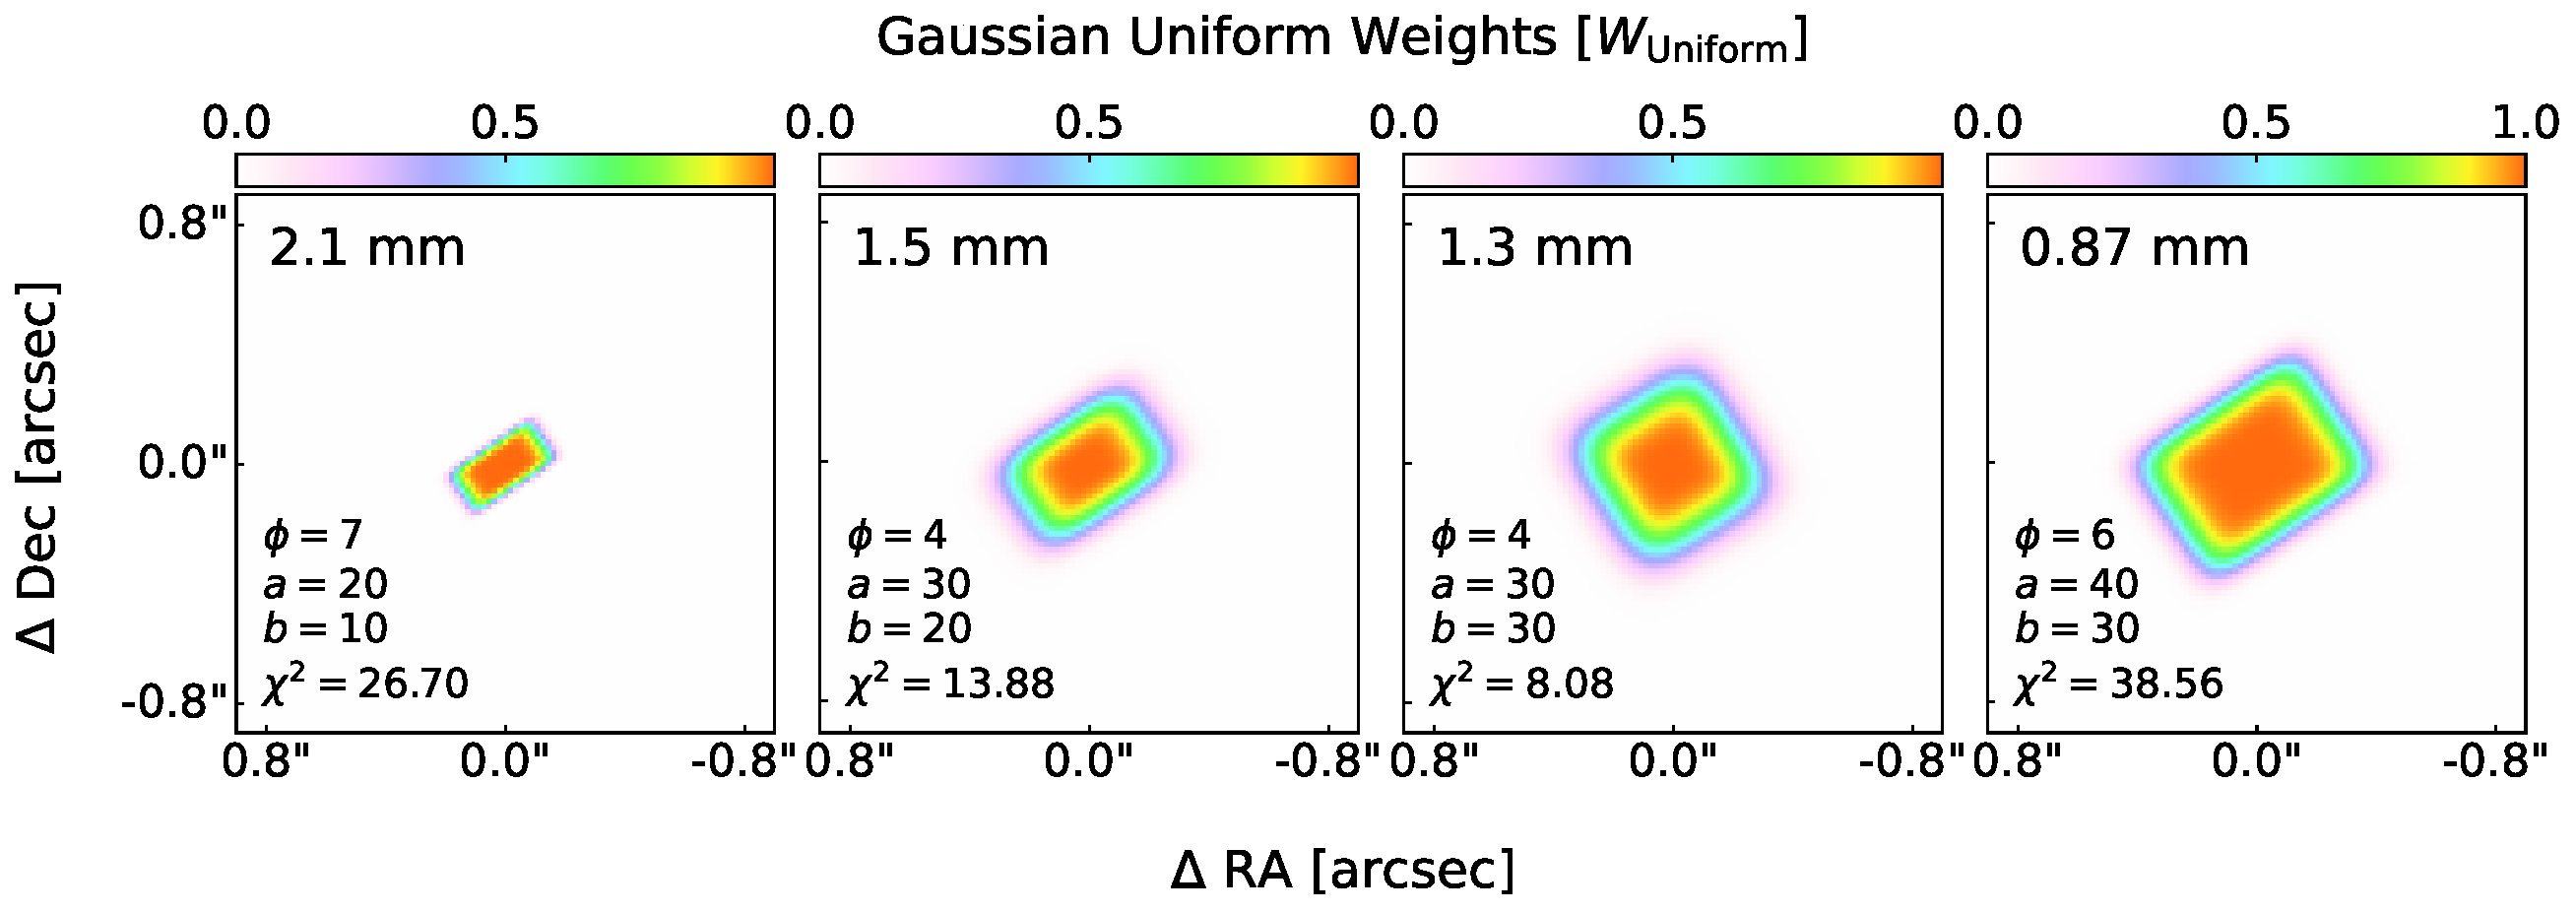
\includegraphics[width=0.99\textwidth]{WRITEUP_AND_IMAGES/IMAGES/WRITEUP/Gaussian/Best_grid_Delta_map.pdf}
  \caption{Maps of the Gaussian uniform weights $W_{\text{uniform}}$ (Equation \ref{eq: gaussian_eq}) for the best-fit Gaussian model for each wavelength, corresponding vector pattern shown in Figure \ref{fig: GaussianBestGrid}. }
  \label{fig: gaussian_best_map_w_uniform}
\end{figure}




The parameter $\Phi$ changes the flatness of the Gaussian, the higher the $\Phi$ value the flatter the Gaussian, transitioning from uniform to azimuthal morphology faster (see Figure \ref{fig: Methods/GaussianExamples}). In the best-fit model at each wavelength, $\Phi$ is greater than 2, producing a flat-topped Gaussian rather than a standard Gaussian. This can also be seen in Figure \ref{fig: gaussian_best_map_w_uniform}, which shows that the area of uniform alignment increases as wavelength decreases. This indicates that uniform alignment, which is consistent with dust self-scattering, contributes more at shorter wavelengths, which is what we expect from Chapter \ref{sec: c4_polarization_maps} and the results from the ratio model. 













% PLOTS
% ----------------------------------------
% ----------------------------------------
% \begin{figure*}[h]
%   \centering

%   % Row 1
%   \begin{minipage}{0.48\textwidth}
%     \centering
%     
\includegraphics[width=\linewidth]{IMAGES/WRITEUP/Gaussian/IRS63_best_gaussian_BAND4.pdf}
%     \textbf{(a) Band 4}
%   \end{minipage}
%   \hfill
%   \begin{minipage}{0.48\textwidth}
%     \centering
%     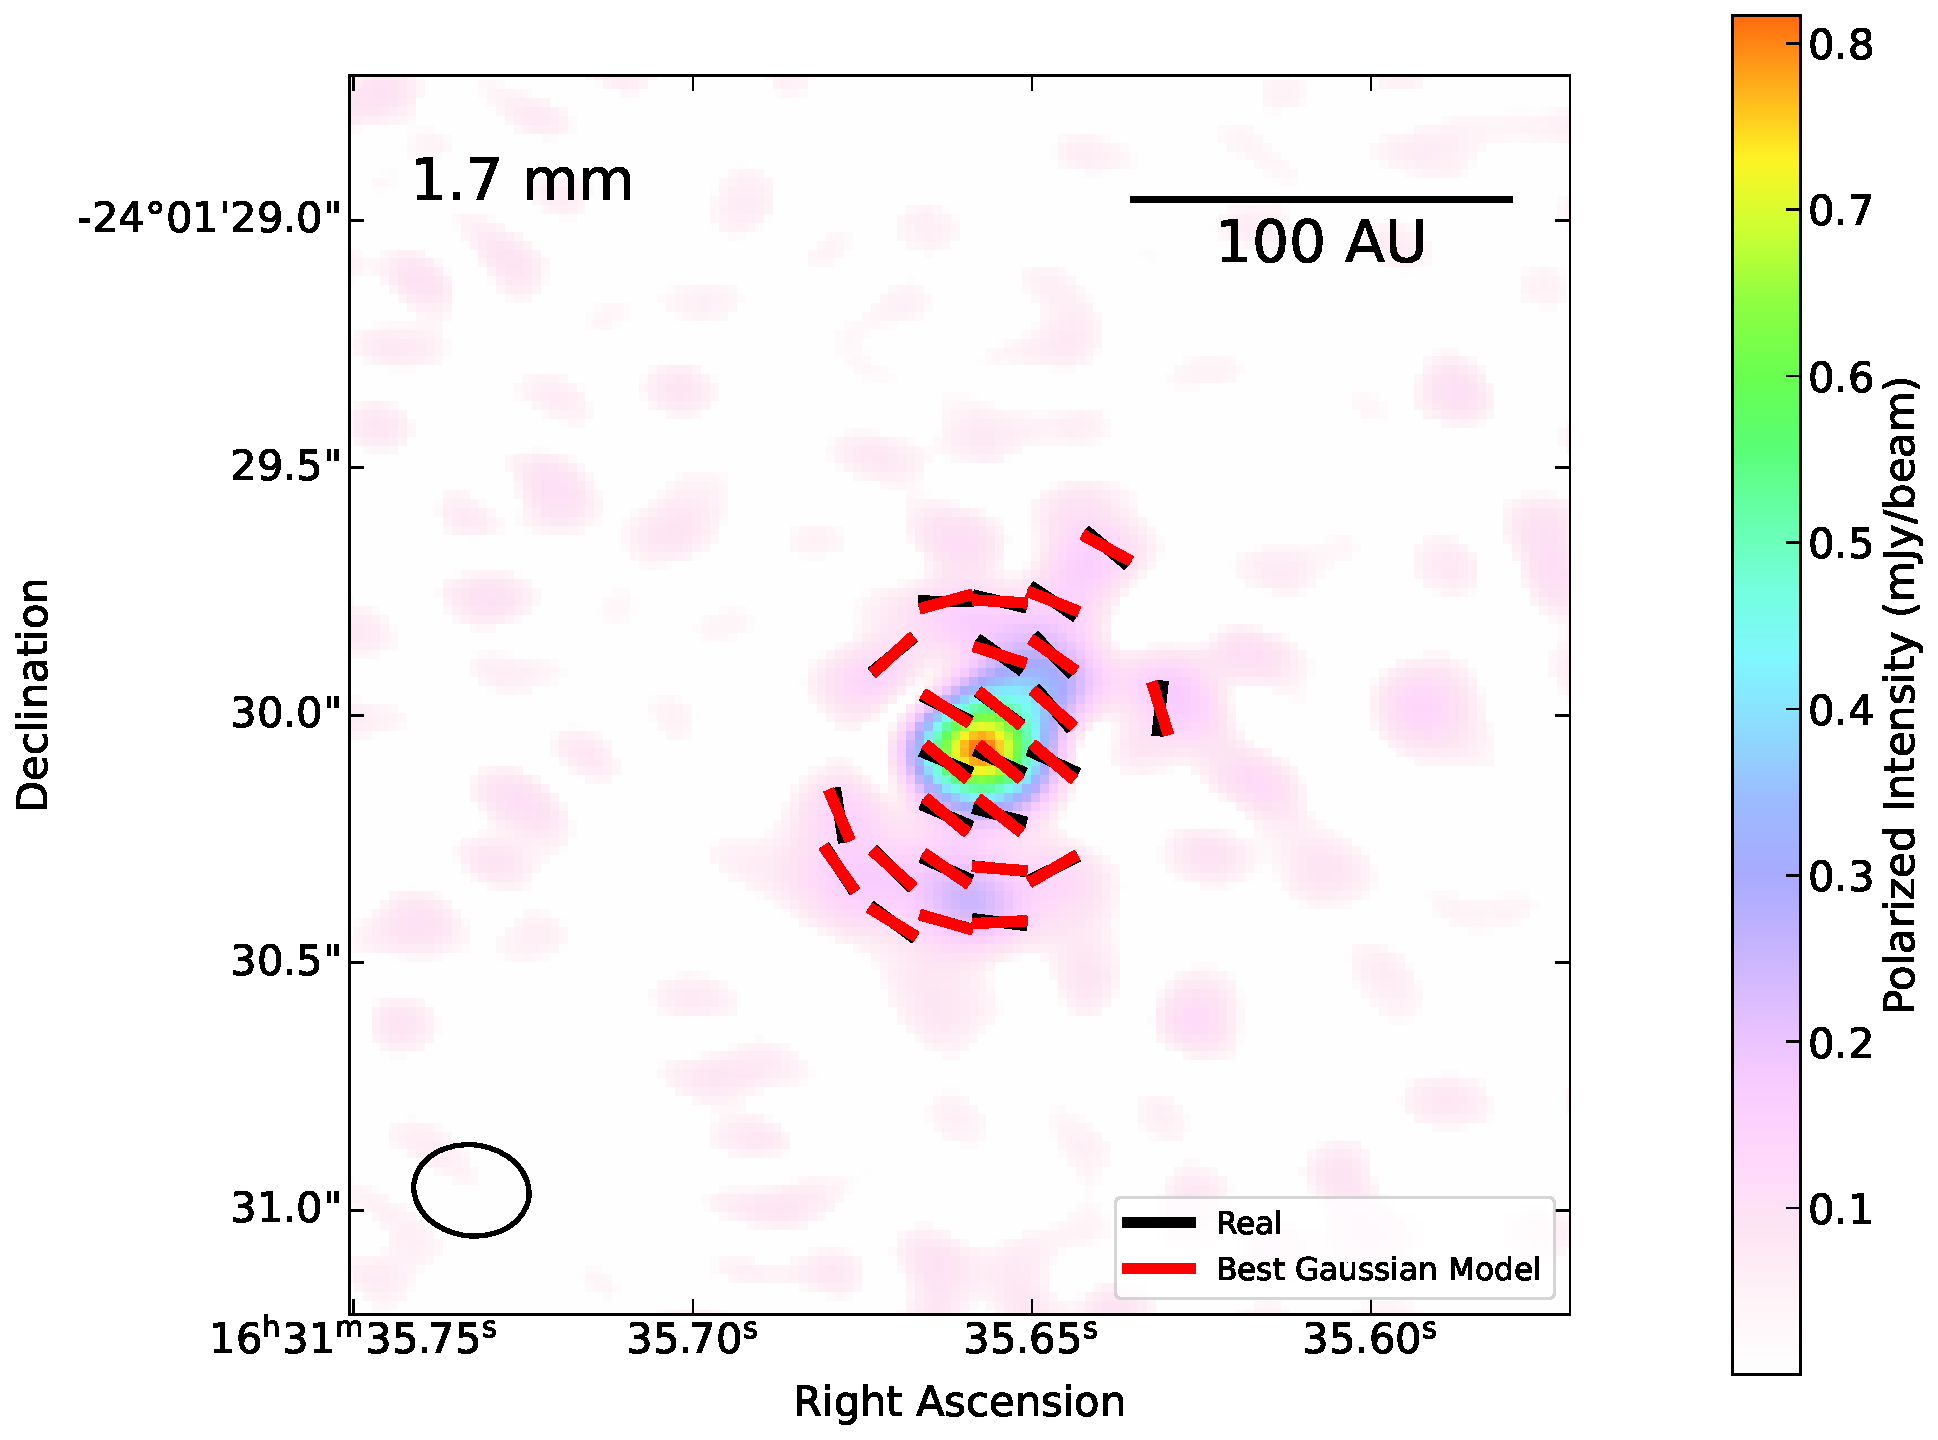
\includegraphics[width=\linewidth]{IMAGES/WRITEUP/Gaussian/IRS63_best_gaussian_BAND5_robust_minus1}
%     \textbf{(b) Band 5}
%   \end{minipage}

%   \vspace{0.5cm}

%   % Row 2
%   \begin{minipage}{0.48\textwidth}
%     \centering
%     
\includegraphics[width=\linewidth]{IMAGES/WRITEUP/Gaussian/IRS63_best_gaussian_BAND6.pdf}
%     \textbf{(c) Band 6}
%   \end{minipage}
%   \hfill
%   \begin{minipage}{0.48\textwidth}
%     \centering
%     
\includegraphics[width=\linewidth]{IMAGES/WRITEUP/Gaussian/IRS63_best_gaussian_BAND7.pdf}
%     \textbf{(d) Band 7}
%   \end{minipage}

%   \caption{
%   \add{caption, make this a grid} \note{Change to $\Delta\alpha$ and $\Delta \delta$ if we chose to do that for other plots.} \note{Update to band 5 robust -1}
%   }

%   \label{fig:best-gaussian-models}
% \end{figure*}
% ----------------------------------------
% ----------------------------------------



